\documentclass[a4paper, 14pt]{extarticle}

% Поля
%--------------------------------------
\usepackage{geometry}
\geometry{a4paper,tmargin=2cm,bmargin=2cm,lmargin=3cm,rmargin=1cm}
%--------------------------------------


%Russian-specific packages
%--------------------------------------
\usepackage[T2A]{fontenc}
\usepackage[utf8]{inputenc} 
\usepackage[english, main=russian]{babel}
%--------------------------------------

\usepackage{textcomp}

% Красная строка
%--------------------------------------
\usepackage{indentfirst}               
%--------------------------------------             


%Graphics
%--------------------------------------
\usepackage{graphicx}
\graphicspath{ {./images/} }
\usepackage{wrapfig}
%--------------------------------------

% Полуторный интервал
%--------------------------------------
\linespread{1.3}                    
%--------------------------------------

%Выравнивание и переносы
%--------------------------------------
% Избавляемся от переполнений
\sloppy
% Запрещаем разрыв страницы после первой строки абзаца
\clubpenalty=10000
% Запрещаем разрыв страницы после последней строки абзаца
\widowpenalty=10000
%--------------------------------------

%Списки
\usepackage{enumitem}

%Подписи
\usepackage{caption} 

%Гиперссылки
\usepackage{hyperref}

\hypersetup {
	unicode=true
}

%Рисунки
%--------------------------------------
\DeclareCaptionLabelSeparator*{emdash}{~--- }
\captionsetup[figure]{labelsep=emdash,font=onehalfspacing,position=bottom}
%--------------------------------------

\usepackage{tempora}

%Листинги
%--------------------------------------
\usepackage{listings}
\lstset{
  basicstyle=\ttfamily\footnotesize, 
  %basicstyle=\footnotesize\AnkaCoder,        % the size of the fonts that are used for the code
  breakatwhitespace=false,         % sets if automatic breaks shoulbd only happen at whitespace
  breaklines=true,                 % sets automatic line breaking
  captionpos=t,                    % sets the caption-position to bottom
  inputencoding=utf8,
  frame=single,                    % adds a frame around the code
  keepspaces=true,                 % keeps spaces in text, useful for keeping indentation of code (possibly needs columns=flexible)
  keywordstyle=\bf,       % keyword style
  numbers=left,                    % where to put the line-numbers; possible values are (none, left, right)
  numbersep=5pt,                   % how far the line-numbers are from the code
  xleftmargin=25pt,
  xrightmargin=25pt,
  showspaces=false,                % show spaces everywhere adding particular underscores; it overrides 'showstringspaces'
  showstringspaces=false,          % underline spaces within strings only
  showtabs=false,                  % show tabs within strings adding particular underscores
  stepnumber=1,                    % the step between two line-numbers. If it's 1, each line will be numbered
  tabsize=2,                       % sets default tabsize to 8 spaces
  title=\lstname                   % show the filename of files included with \lstinputlisting; also try caption instead of title
}
%--------------------------------------

%%% Математические пакеты %%%
%--------------------------------------
\usepackage{amsthm,amsfonts,amsmath,amssymb,amscd}  % Математические дополнения от AMS
\usepackage{mathtools}                              % Добавляет окружение multlined
\usepackage[perpage]{footmisc}
%--------------------------------------

%--------------------------------------
%			НАЧАЛО ДОКУМЕНТА
%--------------------------------------

\begin{document}

%--------------------------------------
%			ТИТУЛЬНЫЙ ЛИСТ
%--------------------------------------
\begin{titlepage}
\thispagestyle{empty}
\newpage


%Шапка титульного листа
%--------------------------------------
\vspace*{-60pt}
\hspace{-65pt}
\begin{minipage}{0.3\textwidth}
\hspace*{-20pt}\centering

\includegraphics[width=\textwidth]{emblem}
\end{minipage}
\begin{minipage}{0.67\textwidth}\small \textbf{
\vspace*{-0.7ex}
\hspace*{-6pt}\centerline{Министерство науки и высшего образования Российской Федерации}
\vspace*{-0.7ex}
\centerline{Федеральное государственное бюджетное образовательное учреждение }
\vspace*{-0.7ex}
\centerline{высшего образования}
\vspace*{-0.7ex}
\centerline{<<Московский государственный технический университет}
\vspace*{-0.7ex}
\centerline{имени Н.Э. Баумана}
\vspace*{-0.7ex}
\centerline{(национальный исследовательский университет)>>}
\vspace*{-0.7ex}
\centerline{(МГТУ им. Н.Э. Баумана)}}
\end{minipage}
%--------------------------------------

%Полосы
%--------------------------------------
\vspace{-25pt}
\hspace{-35pt}\rule{\textwidth}{2.3pt}

\vspace*{-20.3pt}
\hspace{-35pt}\rule{\textwidth}{0.4pt}
%--------------------------------------

\vspace{1.5ex}
\hspace{-35pt} \noindent \small ФАКУЛЬТЕТ\hspace{80pt} <<Информатика и системы управления>>

\vspace*{-16pt}
\hspace{47pt}\rule{0.83\textwidth}{0.4pt}

\vspace{0.5ex}
\hspace{-35pt} \noindent \small КАФЕДРА\hspace{50pt} <<Теоретическая информатика и компьютерные технологии>>

\vspace*{-16pt}
\hspace{30pt}\rule{0.866\textwidth}{0.4pt}
  
\vspace{11em}

\begin{center}
\Large {\bf Лабораторная работа № 9} \\ 
\large {\bf по курсу <<Языки и методы программирования>>} \\
\large <<Перегрузка операций>> 
\end{center}\normalsize

\vspace{8em}


\begin{flushright}
  {Студент группы ИУ9-22Б Волохов А. В. \hspace*{15pt}\\ 
  \vspace{2ex}
  Преподаватель Посевин Д. П.\hspace*{15pt}}
\end{flushright}

\bigskip

\vfill
 

\begin{center}
\textsl{Москва 2023}
\end{center}
\end{titlepage}
%--------------------------------------
%		КОНЕЦ ТИТУЛЬНОГО ЛИСТА
%--------------------------------------

\renewcommand{\ttdefault}{pcr}

\setlength{\tabcolsep}{3pt}
\newpage
\setcounter{page}{2}

\section{Задание}\label{Sect::task}
Данная работа предназначена для изучения возможностей языка C++,
обеспечивающих применение знаков операций к объектам пользовательских типов

Требуется составить шаблон класса,
перегрузив указанные операции. 

Table<T> – таблица, в ячейках которой
размещены значения числового типа T, а
столбцы имеют строковые имена.
Конструктор класса Table<T> должен
формировать пустую таблицу, состоящую из
одного столбца с указанным именем.
Подразумевается, что более сложные таблицы
можно построить из столбцов с помощью
перегруженных операций:
\begin{itemize}
\item «+» – соединение двух таблиц, в
результате которой формируется третья
таблица по следующим правилам:
(a) множество имён столбцов
результирующей таблицы является
объединением множеств имён столбцов
исходных таблиц;
(b) если число строк в одной из
соединяемых таблиц меньше числа строк
во второй, то будем считать, что она
содержит нужное количество строк,
забитых нулями и расположенных внизу
таблицы;
(c) если имеется имя столбца,
присутствующее как в первой из
соединяемых таблиц, так и во второй, то
соответствующий столбец
результирующей таблицы должен
содержать суммы соответствующих
столбцов исходных таблиц;
(d) столбец, имя которого присутствует
только в одной из соединяемых таблиц,
просто копируется в результирующую
таблицу;
\item «%» – добавление в конец таблицы
строки, во всех ячейках которой
находится указанное значение;
\item «[ ]» – получение временного объекта,
обозначающего строку таблицы, к
которому, в свою очередь, может быть
применена операция «[ ]», принимающая
в качестве параметра имя столбца, для
получения ссылки на ячейку строки;
\item «size » – получение количества строк в
таблице;
\item «<<» – вывод таблицы в поток вывода.
\end{itemize}

\section{Результаты}\label{Sect::res}

Исходный код программы представлен в листингах~\ref{lst:code1}--~\ref{lst:code2}--~\ref{lst:code3}.

\begin{figure}[!htb]
\begin{lstlisting}[language={C++},caption={Class Table},label={lst:code1}]
#include <iostream>
#include <vector>
#include <string>
#include <algorithm>

template<typename T>
class Table {
private:
    std::vector<std::string> columnNames;
    std::vector<std::vector<T>> data;

public:
    explicit Table(const std::string& columnName) {
        columnNames.push_back(columnName);
    }

    Table operator+(const Table& other) const {
        Table result = *this;

        for (const auto& columnName : other.columnNames) {
            if (std::find(result.columnNames.begin(), result.columnNames.end(), columnName) == result.columnNames.end()) {
                result.columnNames.push_back(columnName);
            }
        }

        size_t numRows = std::max(result.data.size(), other.data.size());
        result.data.resize(numRows);

        for (size_t i = 0; i < numRows; i++) {
            result.data[i].resize(result.columnNames.size());
        }

        for (size_t col = 0; col < result.columnNames.size(); col++) {
            std::string columnName = result.columnNames[col];
            size_t columnIndex = getColumnIndex(columnName);
            size_t otherColumnIndex = other.getColumnIndex(columnName);

            if (columnIndex != -1 && otherColumnIndex != -1) {
                for (size_t i = 0; i < numRows; i++) {
                    result.data[i][col] = data[i][columnIndex] + other.data[i][otherColumnIndex];
                }
            } else if (otherColumnIndex != -1) {
                for (size_t i = 0; i < numRows; i++) {
                    result.data[i][col] = other.data[i][otherColumnIndex];
                }
            }
        }

        return result;
    }
\end{lstlisting}
\end{figure}
\newpage
\begin{figure}[!htb]
\begin{lstlisting}[language={C++},caption={Class Table (продолжение)},label={lst:code2}]
Table& operator%(const T& value) {
        std::vector<T> newRow(columnNames.size(), value);
        data.push_back(newRow);

        return *this;
    }

    std::vector<T>& operator[](size_t rowIndex) {
        return data[rowIndex];
    }

    [[nodiscard]] size_t size() const {
        return data.size();
    }

    friend std::ostream& operator<<(std::ostream& os, const Table& table) {
        for (const auto& columnName : table.columnNames) {
            os << columnName << '\t';
        }
        os << '\n';

        size_t numRows = table.size();
        size_t numColumns = table.columnNames.size();
        for (size_t row = 0; row < numRows; row++) {
            for (size_t col = 0; col < numColumns; col++) {
                os << table.data[row][col] << '\t';
            }
            os << '\n';
        }

        return os;
    }


private:
    [[nodiscard]] int getColumnIndex(const std::string& columnName) const {
        auto it = std::find(columnNames.begin(), columnNames.end(), columnName);

        if (it != columnNames.end()) {
            return std::distance(columnNames.begin(), it);
        }

        return -1;
    }
};
\end{lstlisting}
\end{figure}
\begin{figure}[!htb]
\begin{lstlisting}[language={C++},caption={Main (в том же файле)},label={lst:code3}]
int main() {
    Table<int> table1("Column1");
    table1 % 10;
    table1 % 20;
    table1 % 30;

    Table<int> table2("Column2");
    table2 % 100;
    table2 % 200;
    table2 % 300;
    table2 % 100;

    Table<int> table3 = table1 + table2;

    std::cout << table3 << std::endl;
    std::cout << table3[0][1] << std::endl;
    std::cout << table3.size() << std::endl;

    Table<int> table4("Column1");
    table4 % 1;
    table4 % 2;
    table4 % 3;
    table4 % 4;

    table4 = table3 + table4;
    std::cout << table4 << std::endl;

    return 0;
}
\end{lstlisting}
\end{figure}

\newpage



\begin{figure}[!htb]
	\centering
	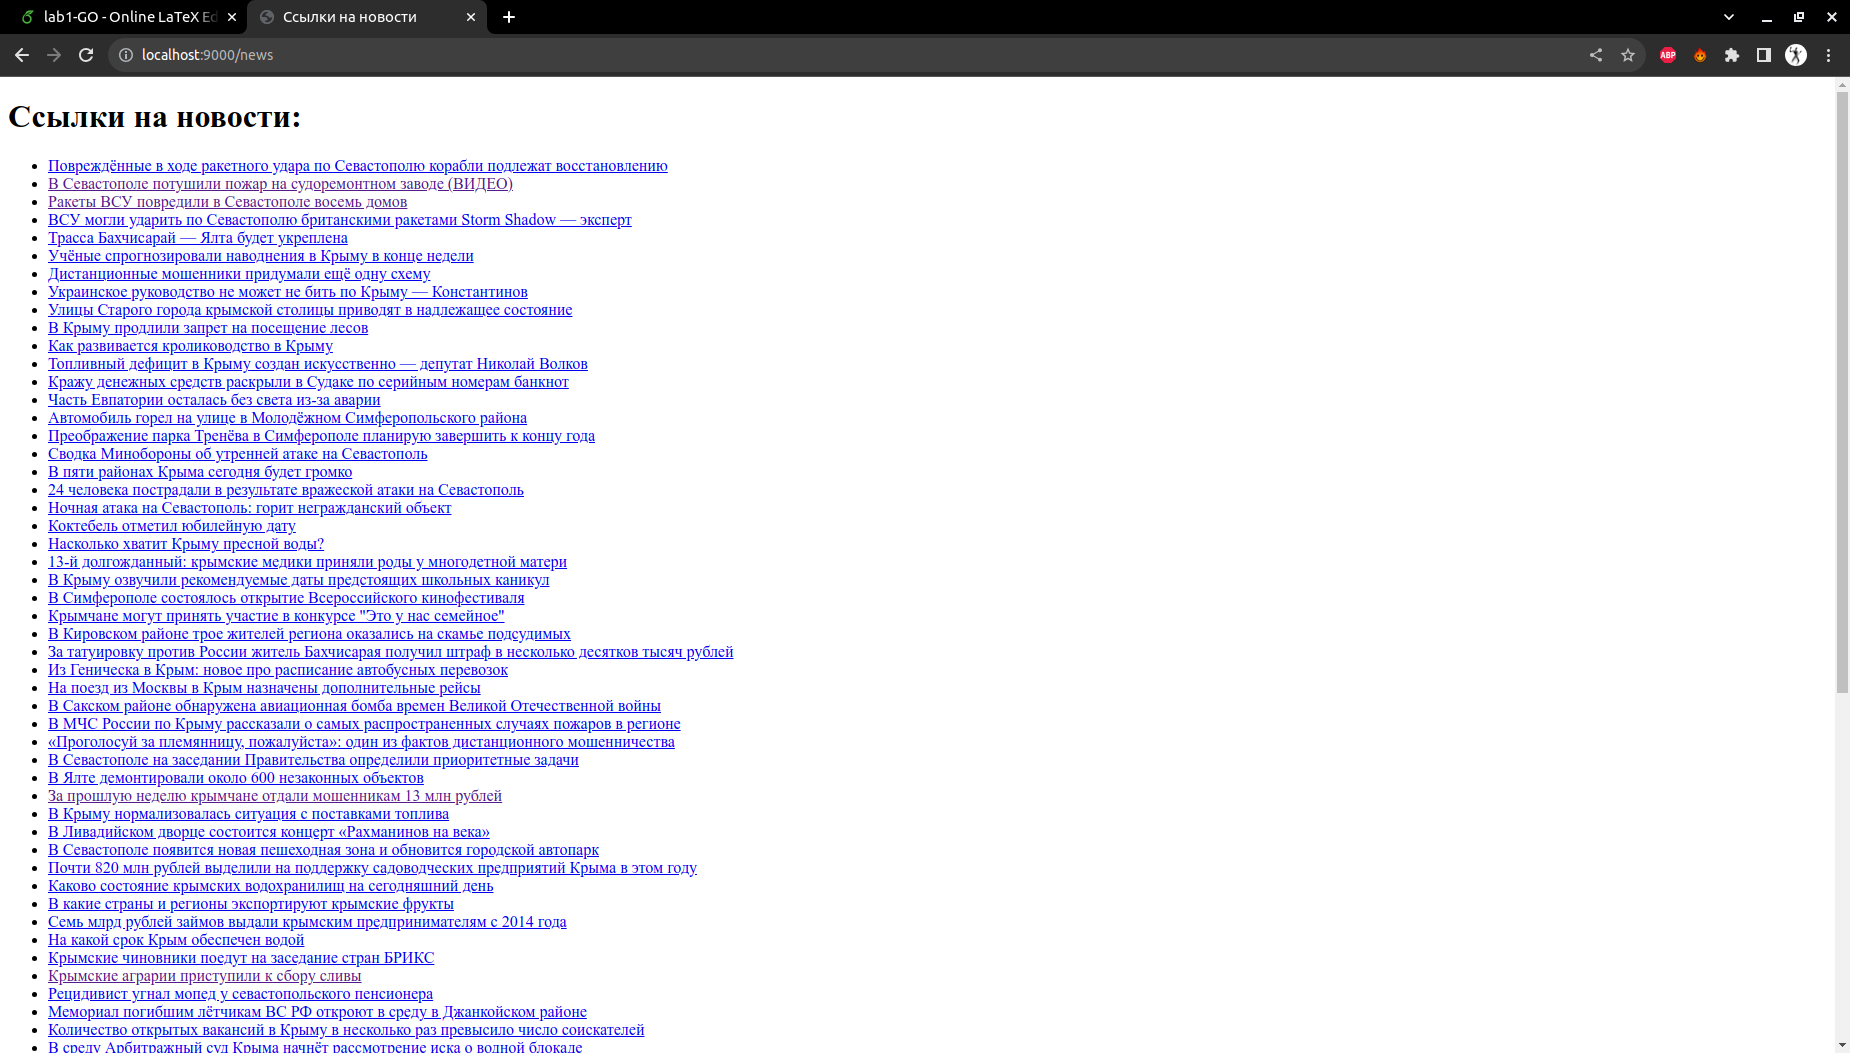
\includegraphics[width=0.8\textwidth]{result.png}
\caption{Результат}
\label{fig:img1}
\end{figure}





\end{document}
